%!TEX root = AllegThesis.tex
%
% $Id: ch02_relatedwork
%
\chapter{Tracker Electronics Corrections}\label{ch:trackerelectronics}

In the summer of 2015, the Mu2e group obtained a prototype of a subset of the tracker. This provided some of the first opportunities to study the straw electronics response and compare it to simulations. In this chapter, several of these measurements using the ADC output are presented, many of which have been used to compare to and update the current Mu2e simulations.

\section{Low Energy Waveforms}

When a particle passes through a straw, it ionizes charge which then produces an impulse of current on the straw wire. This current is then shaped by the electronics and digitized by the ADC. Although, the shaping is in reality much more complex, it has been modeled as a simple RC CR circuit. With this assumption, a signal of the form 
\begin{equation}
	V(t) = V_0 \frac{t}{\tau^2} e^{-t / \tau}
	\label{eq:base1}
\end{equation}
\begin{figure}[htp!]
    \centering
    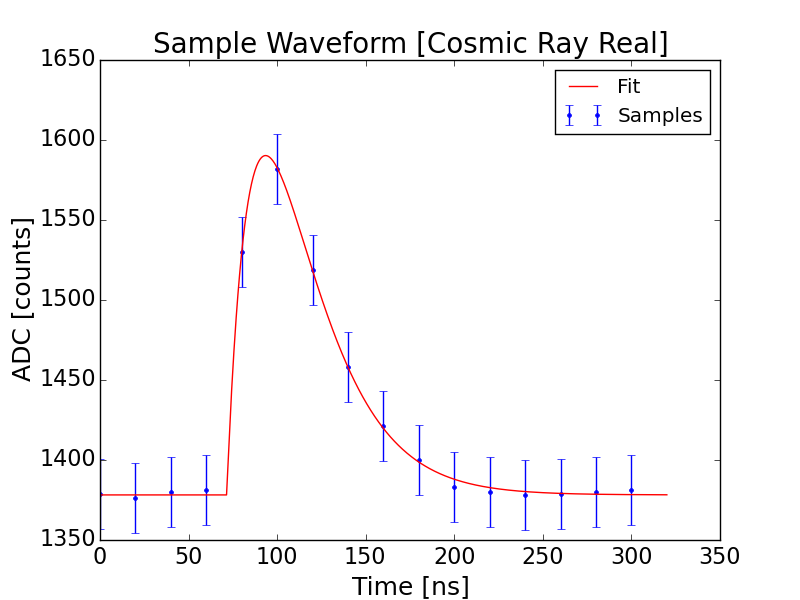
\includegraphics[scale=0.5]{Images2/sampleWaveformCosmic.png}
    \caption{Sample waveform of cosmic muon from ADC output.}
    \label{fig:sampleCosmic}
\end{figure} 
is obtained, where $\tau$ defines the shaping time, and $V_0$ is constant which depends on the amount of energy deposited by a given particle. A sample waveform is shown in Figure \ref{fig:sampleCosmic} with a fit to this model superimposed. 

The source used to produce this waveform was
cosmic-ray muons. These muons are classified as minimum ionizing particles (mip's). Consequently, they should have a similar $dE/dx$ and thus deposit energy in a similar manner to electrons in the actual experiment.

Qualitatively, there is good agreement between this simple model and the prototype waveforms. This provides some validation to the electronics model in the simulations. ???

\section{Shaping Time}
In the current simulations, the default value for the shaping time has been fixed to $25$ ns, a value based on prior SPICE simulations. To more finely tune this parameter an Iron-55 source used. Fe-55, emits photons which have a very precise-value for their energy, and produce a single cluster of ionizations. This local cluster of ionizations well-approximates a current impulse. This is in contrast to massive particles which produces a path of ionizations that reach straw wire over a range of time. By fitting Equation \ref{eq:base1} to Fe-55 waveforms, with $\tau$ as a free parameter we can determine a more precise value for this parameter. Figure ... shows the distribution of this fit parameter, with a peak near $22$ ns and a reasonable small spread. This value has been added as the default to the Mu2e simulations.

\section{ADC Gain and Noise}

\subsection{ADC Gain}

\begin{figure}[htp!]
    \centering
    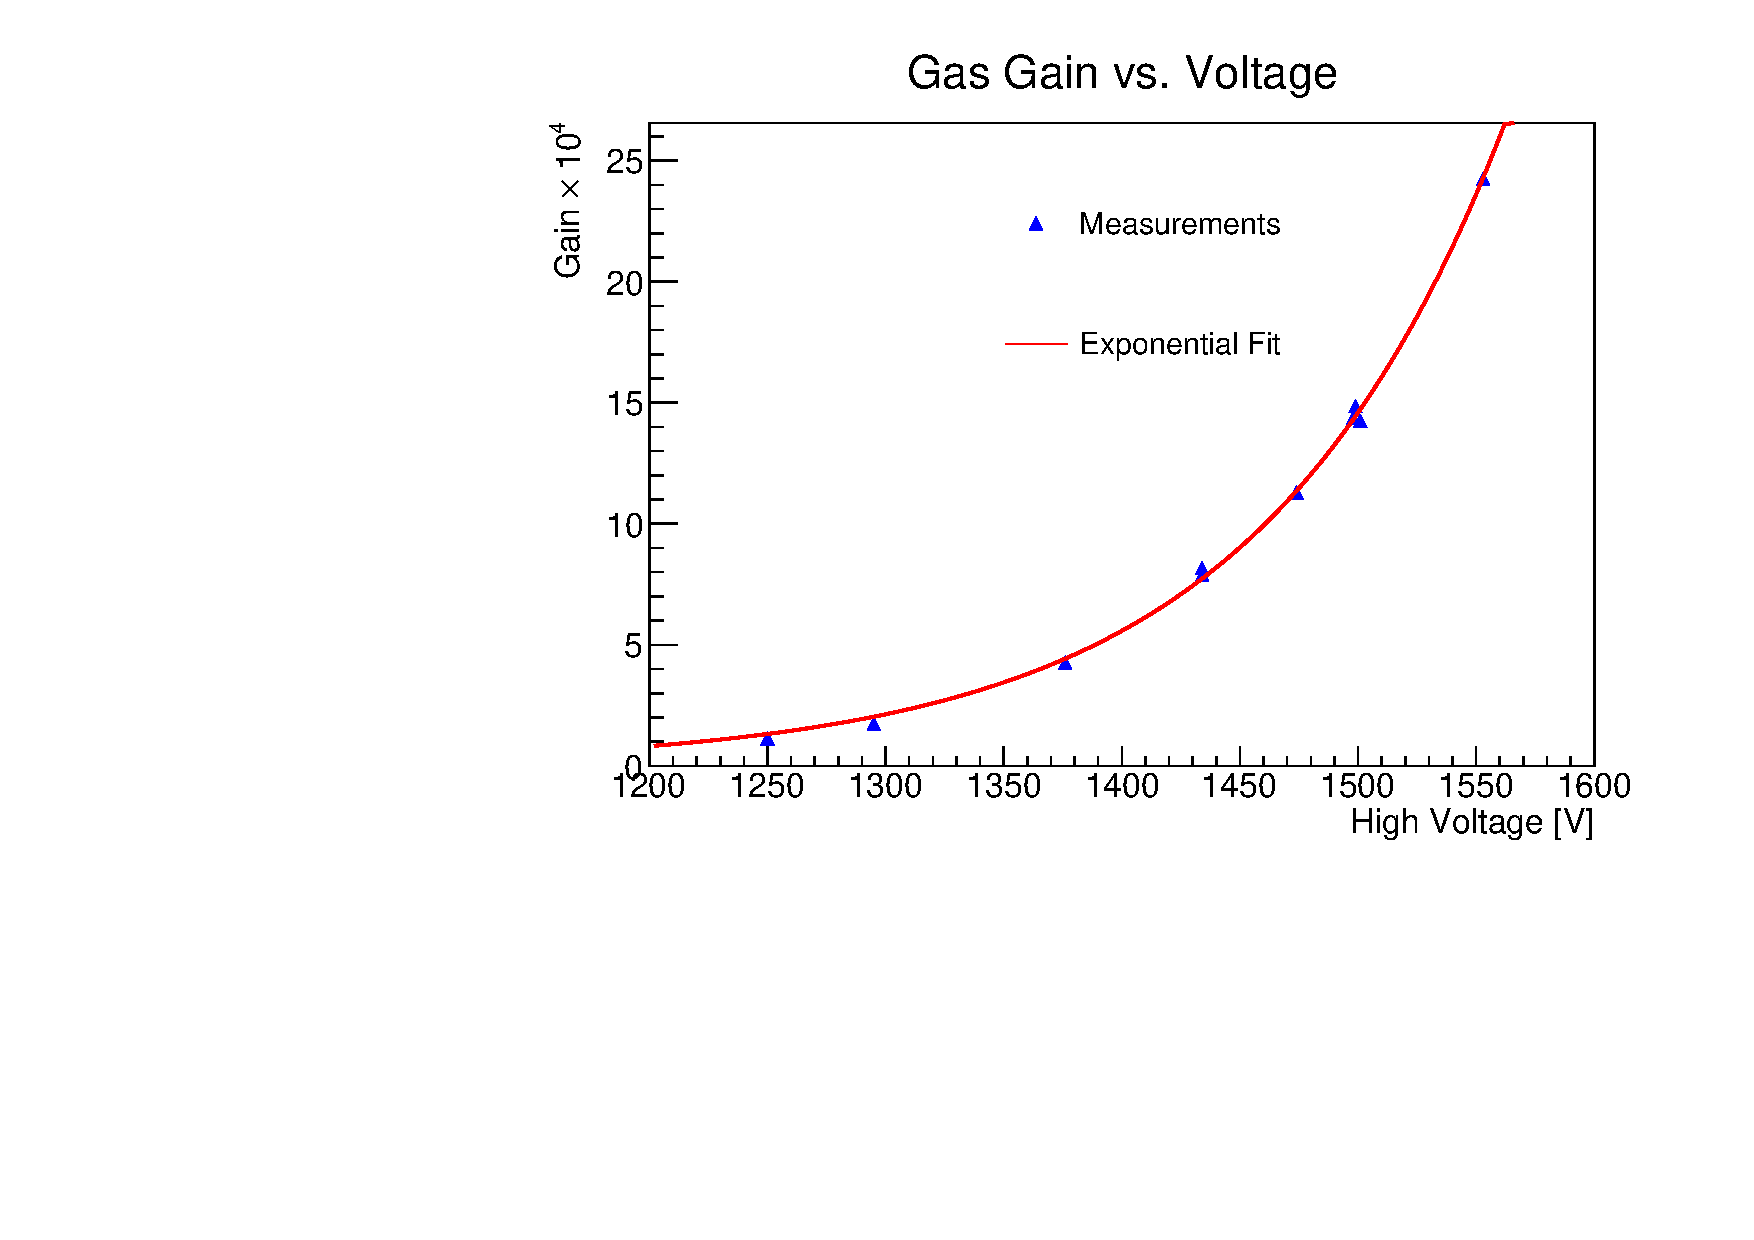
\includegraphics[scale=0.5]{Images2/gasGainVsVoltage.pdf}
    \caption{Gas gain as a function of high voltage.}
    \label{fig:gasGain}
\end{figure} 
When the current impulse reaches the wire, it is not only shaped but also magnified by a preamp. This corresponds to a vertical scaling of the ADC waveform. 
%A part of the amplification results from the chain reaction of ionizations that occur in the gas as the incident particle pass through the straw. A second amplification occurs purely from amplifiers contained in the straw electronics. The first amplification (which we define as the gas gain) has been found through previous measurements to be related to the high voltage across the straws. This relationship is shown in Figure \ref{fig:gasGain}. 
We can measure this amplification (defined to be the electronics gain) once again by using Fe-55 data. The advantage to using Fe-55 is that the 5.9 keV peak in it's energy spectrum is well-defined in Geant4, which can easily be simulated in Mu2e Offline. 

Given the energy deposited by a single photon ($E_{\gamma}$) from the Fe-55 source and knowing computing the energy per ionization ($E_{ionization}$) using Geant4 then the voltage outputted by the ADC is given by
\begin{equation}
	 \frac{E_{\gamma}}{E_{ionization}} \times {Gain_{gas}} \times Gain_{electronics} = V_{ADC}
	 \label{eq:electronicsGain}
\end{equation}
The gas gain ($Gain_{gas}$) is defined to be the scaling resulting from the chain reaction of ionizations that occur in the gas as the incident particle pass through the straw. This amplification has been found through previous measurements to be related to the high voltage across the straws (shown in Figure \ref{fig:gasGain}). 

By measuring energy spectrum of the Fe-55 waveforms using the prototype, we can compute $V_{ADC}$ which corresponds to the voltage at the peak and scale this value to find the corresponding electronics gain.

\subsection{ADC Noise}

By studying the width of the peak, we can also estimate the noise in the signal. Sources of noise affecting the ADC output, include gain variation, smearing from the ADC sampling rate, and electronics noise. This noise will increase the variation of the ADC output which will widen the width of the peak. We can estimate the amount of noise by varying the noise in the simulation to match the width seen in the prototype data. Doing this, the noise was measured to be approximately 8 mV. Figure ... shows a comparison of the spectrums for Fe55 using both the prototype and simulations. After tuning the electronics gain and noise, the spectrum for the 5.9 keV peak match. On a side note, below the 5.9 keV there is less agreement between the simulations and data. This is because Geant4 currently does not currently simulate the 2.9 keV escape peak.

\section{Threshold Gain and Noise}

In the straw electronics a threshold is applied so that only signals of a certain amplitude are outputted by the ADC. This is important for reducing the amount of low energy noise from signals of interest. Theoretically, the threshold should form a step-function in acceptance, eliminating all signals below the threshold while accepting all signals above. Due to noise this response is in reality much more smooth. To measure this, the Iron-55 spectrum was measured at two different thresholds (Figure \ref{fig:peakMinusPedThresh}). The ratio of these two spectrums produces precisely the threshold response (Figure \ref{fig:relativeRates}).

\begin{figure}[htp!]
    \centering
    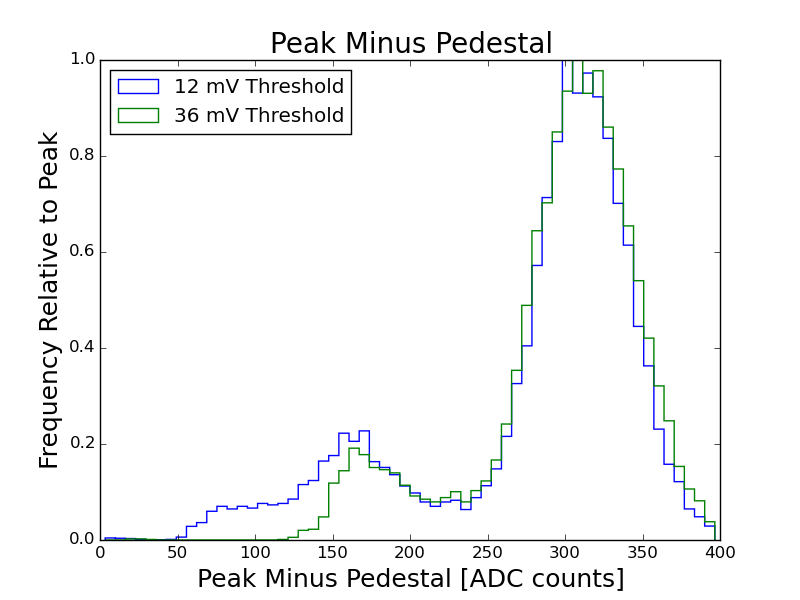
\includegraphics[scale=0.5]{Images2/peakMinusPedThresh.png}
    \caption{Peak minus pedestal for 12 mV and 36 mV thresholds.}
    \label{fig:peakMinusPedThresh}
\end{figure} 
\begin{figure}[htp!]
    \centering
    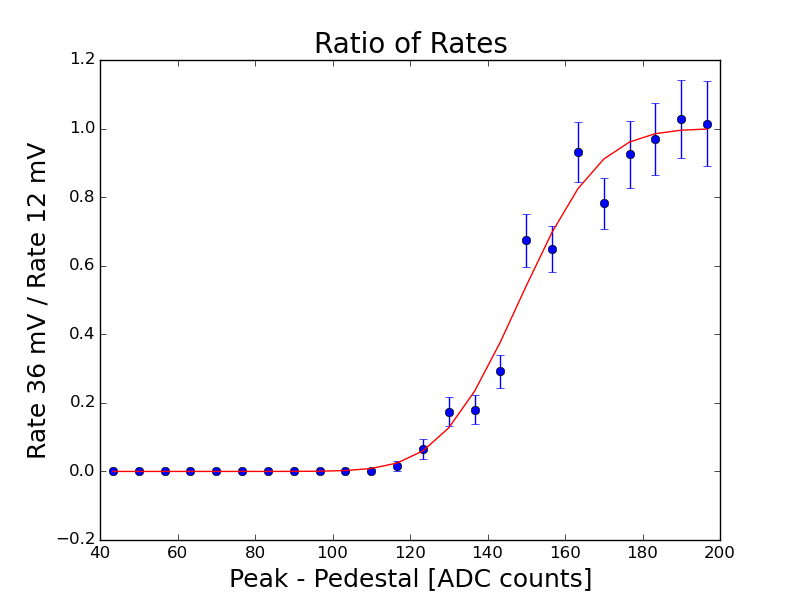
\includegraphics[scale=0.5]{Images2/relativeRates.png}
    \caption{Ratio of peak minus pedestal for 12 mV and 36 mV.}
    \label{fig:relativeRates}
\end{figure} 


As expected, the ratio forms a smooth step function. This data was fitted to the functional form
\begin{equation}
    g(x; a,b) = \frac{\text{erf}\left( a(x - b) + 1 \right)}{2}
\end{equation}
Note that $a$ defines the threshold which the ratio is $1/2$. $b$ in the other hand defines the spread in the function, and hence provides a estimate for the noise in the threshold channels.



\section{Preamp Saturation \label{sec:preampSaturation}}
The straw electronics contains a preamp. At voltages this component is useful for amplifying the signal. However, for higher voltages the preamp saturates. Measuring the levels at which saturation occur are important for reducing crosstalk between straws. In otherwords, if the saturation level is too high (which can result from proton background), signals in one straw may become large enough that the corresponding signals induced in neighboring straws may overwhelm signals of interest. 

Like in the previous studies an Fe-55 source was used. %Given the energy deposited by Fe-55 we can compute the corresponding number of ionizations. This in turn can be used to compute the charge deposited on the straw wires, which is directly proportional to the current and hence to the voltage measured in the ADC output. The full relationship between the energy deposited and the resultant charge on the straw is shown in Equation \ref{eq:electronicsGain}.
Given the High Voltage, with Equation \ref{eq:electronicsGain} we can compute an estimate for the voltage measured with the ADC in the linear regime. Thus, for voltages in this linear region we expect this estimate to match what is the value measured with the protype. However, by comparing this estimate over a wider range of voltages we can determine where the preamp response becomes nonlinear and saturates.

\begin{figure}[htp!]
    \centering
    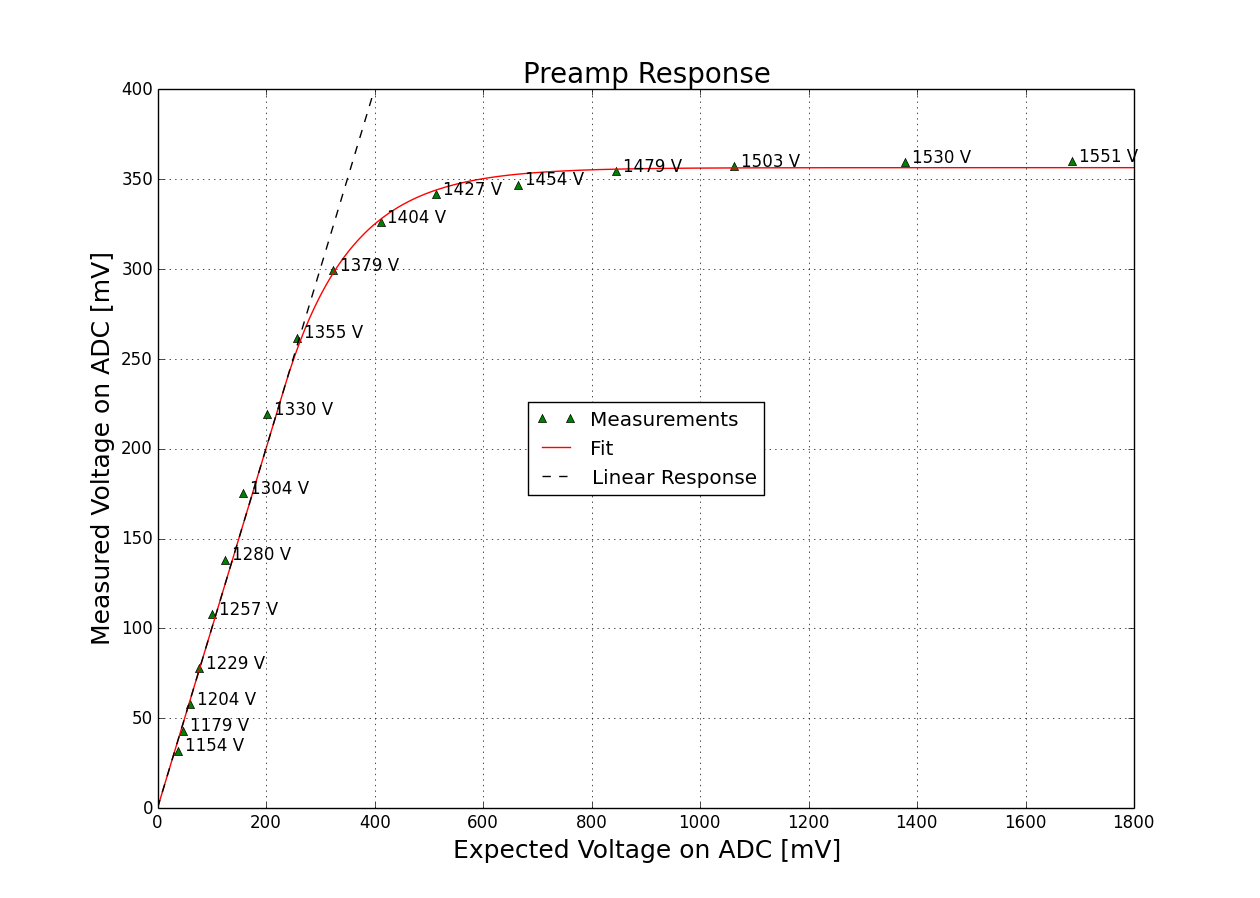
\includegraphics[scale=0.4]{Images2/preampResponse.png}
    \caption{Preamp response over a range of high voltages.}
    \label{fig:preampResponse}
\end{figure} 

Figure \ref{fig:preampResponse} shows the measured voltage versus the computed voltage over a wide range of frequencies. This response was fit to the model 
%Figure ... shows the relationship between the ADC output versus the deposited charge. As expected, for lower voltages the response is clearly linear. By fitting a line to the linear regime, the scaling factor between the resultant voltage from the ADC and the deposited charge was found to be ...
%Rescaling the charge by this value, Figure ... shows the preamp response purely as a function of voltage. The response was fit to the model
\begin{equation}
	f(V; V_{sat}, V_{max}) = \begin{cases} 
		V & V < V_{sat} \\
		V_{sat} + (V_{max} - V_{sat}) e^{-\frac{V - V_{max}}{V_{sat - V_{max}}} } & V \geq V_{sat} \\
		\end{cases} 
\end{equation}
where $V_{sat}$ is the threshold at which the preamp response becomes nonlinear and $V_{max}$ is the maximum response for any voltage. 

The resultant fit parameters were $V_{max} = 356 mV$ and $V_{sat} = 234 mV$, which have been incorporated into the Mu2e simulation. The dynamic range of the preamp is $1500 mV$ which is significantly greater than $V_{max}$. In Section \ref{sec:sat} methods are developed to recover much of the dynamic range from the ADC waveforms. 

\section{High Energy Corrections}

All the studies so far have been succesfully implemented into Mu2e Offline. For this final study significant process has been made. However, further work is still needed before it can be incorporated the Mu2e framework.

Prior to the studies using the prototype all waveforms were predicted to be of the form in Equation \ref{eq:base1}. With the prototype at Low Energies this function appeared to hold true. However, for higher energy pulses an undershoot begins to appear (Figure ...). Most of the waveforms resulting from conversion lie in the lower energy regime. This undershoot is prevalent in many proton signals. Depending on the decay time of this undershoot, it is possible for this additional feature to overwhelm a following conversion electron signal. In other words, the undershoot will place limits on the dead time of the ADC ???

In addition, the undershoot will restrict possible energy reconstruction methods. In particular, the current method used to reconstruct the energy deposited by a waveform involves summing the ADC values and subtracting the pedestal. However, for waveforms with large undershoots, the estimated energy will be severely reduced. Thus other methods, such as computing the difference between the peak value and the pedestal or a fitting method must be used. 

To model this extra feature a current waveform is added to Equation \ref{eq:basefit} of the form 
\begin{equation}
	U(t;t_0,n,\xi) = - U_0 \left( \frac{t - t_0}{\xi n} \right)^n e^{-(t - t_0 - \xi n)/\xi }
\end{equation}
The total waveform is thus $V(t) + U(t;t_0,n,\xi)$. The functional form of $U(t;t_0,n,\xi)$ is very similar to a negated version of $V(t)$, with some subtle changes in the parameters:
\begin{itemize}
\item Similar to $\tau$ in $V(t)$, $\xi$ describes the decay time back to pedestal. 
\item $t_0$ defines the time at which the undershoot first appears with respect to the start in $V(t)$.
\item Normalization is chosen so that the minimum occurs at $U_0$. For $V(t)$, normalization was chosen so that the integral of $V(t)$ from zero to infinity was $V_0$.
\item $n$ defines the power of the term which is polynomial in $t$. Consequently, the minimum of $U$ occurs at $t = \xi n$. For comparison, the maximum of $V_0$ is constrained to $t = \tau$.
\end{itemize}


An example waveform is shown in Figure ... This method reasonably models the general shape of the waveform and consequently could be incorporated into energy reconstruction methods (see Chapter \ref{ch:implem}). However, it is not so clear how best to implement this model into the simulations. In the simulations for each hit subsets of the charge (called hitlets) are individually shaped and the resultant waveforms are summed linearly. The undershoot though is a inherently time-dependent effect and does not scale linearly with charge. At the moment, the candidate implemention is to add these small undershoots to each hitlet and like before simply sum up all these individual response. This is not without drawbacks, and has yet to be fully implemented (What are the drawbacks???). For more precise simulations a more complex model of the straws electronics will be necessary.

pixel/mu2e/allruns/lbl-cosmics


